\documentclass[10pt]{article}
\usepackage[paperwidth=11.8cm,paperheight=4.5cm,margin=0pt]{geometry}
\usepackage{amsmath,amssymb}
\usepackage{mathptmx}
\renewcommand{\hbar}{\mathchar'26\mkern-9mu h}
\usepackage{tikz}
\pagestyle{empty}
\begin{document}
\special{papersize=11.8cm,4.5cm}
\noindent
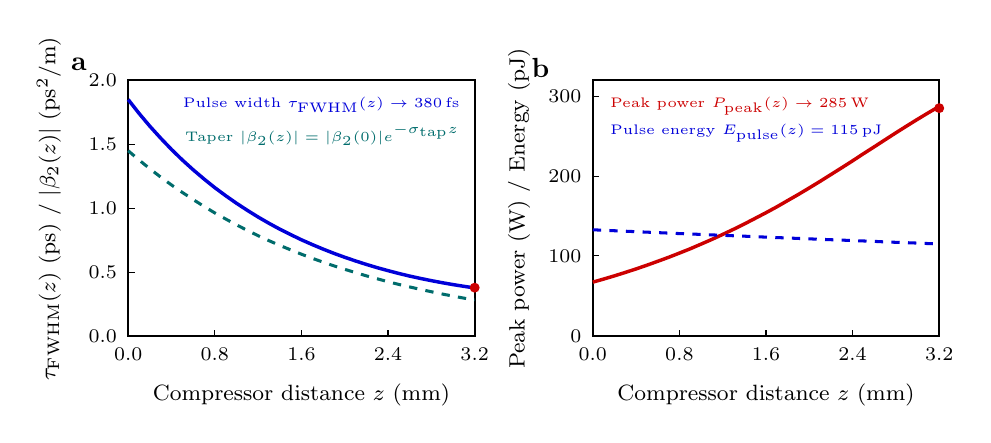
\begin{tikzpicture}[x=1cm,y=1cm,font=\footnotesize]
  % Panel a: Pulse FWHM compression & exponential dispersion taper along InGaAs waveguide
  \node[anchor=north west,font=\bfseries\normalsize] at (0.10,4.35) {a};
  \draw[thick] (0.95,0.70) rectangle (5.35,3.95);
  \foreach \v/\y in {0.0/0.70, 0.5/1.51, 1.0/2.32, 1.5/3.14, 2.0/3.95} {
    \draw (0.95,\y) -- (1.03,\y);
    \node[left,font=\scriptsize] at (0.93,\y) {\v};
  }
  \foreach \xval/\xpos in {0.0/0.95, 0.8/2.05, 1.6/3.15, 2.4/4.25, 3.2/5.35} {
    \draw (\xpos,0.70) -- (\xpos,0.78);
    \node[below,font=\scriptsize] at (\xpos,0.68) {\xval};
  }
  \node[below,font=\footnotesize] at (3.15,0.22) {Compressor distance $z$ (mm)};
  \node[rotate=90,above,font=\footnotesize] at (0.22,2.32) {$\tau_{\mathrm{FWHM}}(z)$ (ps) / $|\beta_2(z)|$ ($\mathrm{ps^2/m}$)};

  \draw[blue!85!black,line width=1.25pt] (0.950,3.706) -- (1.087,3.531) -- (1.225,3.367) -- (1.363,3.215) -- (1.500,3.072) -- (1.637,2.939) -- (1.775,2.814) -- (1.913,2.697) -- (2.050,2.587) -- (2.188,2.485) -- (2.325,2.389) -- (2.463,2.299) -- (2.600,2.214) -- (2.737,2.135) -- (2.875,2.060) -- (3.013,1.991) -- (3.150,1.925) -- (3.288,1.864) -- (3.425,1.807) -- (3.562,1.753) -- (3.700,1.703) -- (3.838,1.656) -- (3.975,1.612) -- (4.112,1.571) -- (4.250,1.533) -- (4.388,1.497) -- (4.525,1.464) -- (4.663,1.434) -- (4.800,1.406) -- (4.938,1.380) -- (5.075,1.356) -- (5.213,1.334) -- (5.350,1.313);
  \draw[teal!85!black,dashed,line width=1.1pt] (0.950,3.056) -- (1.087,2.939) -- (1.225,2.827) -- (1.363,2.721) -- (1.500,2.621) -- (1.637,2.527) -- (1.775,2.436) -- (1.913,2.349) -- (2.050,2.266) -- (2.188,2.189) -- (2.325,2.115) -- (2.463,2.044) -- (2.600,1.977) -- (2.737,1.914) -- (2.875,1.854) -- (3.013,1.797) -- (3.150,1.742) -- (3.288,1.690) -- (3.425,1.641) -- (3.562,1.594) -- (3.700,1.550) -- (3.838,1.508) -- (3.975,1.467) -- (4.112,1.430) -- (4.250,1.392) -- (4.388,1.358) -- (4.525,1.326) -- (4.663,1.295) -- (4.800,1.265) -- (4.938,1.236) -- (5.075,1.210) -- (5.213,1.184) -- (5.350,1.161);
  \fill[red!80!black] (5.350,1.317) circle (1.8pt);

  \node[anchor=north east,font=\tiny,blue!85!black] at (5.28,3.86) {Pulse width $\tau_{\mathrm{FWHM}}(z) \to 380\,\mathrm{fs}$};
  \node[anchor=north east,font=\tiny,teal!85!black] at (5.28,3.52) {Taper $|\beta_2(z)| = |\beta_2(0)|e^{-\sigma_{\mathrm{tap}}z}$};

  % Panel b: Peak power P_peak(z) and pulse energy E_pulse(z)
  \node[anchor=north west,font=\bfseries\normalsize] at (5.95,4.35) {b};
  \draw[thick] (6.85,0.70) rectangle (11.25,3.95);
  \foreach \v/\y in {0/0.70, 100/1.72, 200/2.73, 300/3.75} {
    \draw (6.85,\y) -- (6.93,\y);
    \node[left,font=\scriptsize] at (6.83,\y) {\v};
  }
  \foreach \xval/\xpos in {0.0/6.85, 0.8/7.95, 1.6/9.05, 2.4/10.15, 3.2/11.25} {
    \draw (\xpos,0.70) -- (\xpos,0.78);
    \node[below,font=\scriptsize] at (\xpos,0.68) {\xval};
  }
  \node[below,font=\footnotesize] at (9.05,0.22) {Compressor distance $z$ (mm)};
  \node[rotate=90,above,font=\footnotesize] at (6.18,2.32) {Peak power (W) / Energy (pJ)};

  \draw[red!80!black,line width=1.25pt] (6.850,1.387) -- (6.987,1.426) -- (7.125,1.467) -- (7.262,1.510) -- (7.400,1.555) -- (7.537,1.602) -- (7.675,1.652) -- (7.812,1.702) -- (7.950,1.756) -- (8.088,1.811) -- (8.225,1.870) -- (8.363,1.930) -- (8.500,1.993) -- (8.637,2.058) -- (8.775,2.126) -- (8.912,2.197) -- (9.050,2.269) -- (9.188,2.344) -- (9.325,2.423) -- (9.463,2.502) -- (9.600,2.584) -- (9.738,2.668) -- (9.875,2.754) -- (10.012,2.840) -- (10.150,2.928) -- (10.287,3.018) -- (10.425,3.106) -- (10.562,3.195) -- (10.700,3.284) -- (10.838,3.371) -- (10.975,3.456) -- (11.113,3.539) -- (11.250,3.619);
  \draw[blue!85!black,dashed,line width=1.1pt] (6.850,2.052) -- (6.987,2.046) -- (7.125,2.040) -- (7.262,2.034) -- (7.400,2.028) -- (7.537,2.022) -- (7.675,2.016) -- (7.812,2.010) -- (7.950,2.004) -- (8.088,1.999) -- (8.225,1.993) -- (8.363,1.987) -- (8.500,1.982) -- (8.637,1.976) -- (8.775,1.971) -- (8.912,1.964) -- (9.050,1.959) -- (9.188,1.953) -- (9.325,1.948) -- (9.463,1.942) -- (9.600,1.937) -- (9.738,1.931) -- (9.875,1.926) -- (10.012,1.921) -- (10.150,1.915) -- (10.287,1.910) -- (10.425,1.905) -- (10.562,1.898) -- (10.700,1.893) -- (10.838,1.888) -- (10.975,1.883) -- (11.113,1.877) -- (11.250,1.872);
  \fill[red!80!black] (11.250,3.597) circle (1.8pt);

  \node[anchor=north west,font=\tiny,red!80!black] at (6.95,3.86) {Peak power $P_{\mathrm{peak}}(z) \to 285\,\mathrm{W}$};
  \node[anchor=north west,font=\tiny,blue!85!black] at (6.95,3.52) {Pulse energy $E_{\mathrm{pulse}}(z) = 115\,\mathrm{pJ}$};
\end{tikzpicture}
\end{document}
